% Options for packages loaded elsewhere
\PassOptionsToPackage{unicode}{hyperref}
\PassOptionsToPackage{hyphens}{url}
\PassOptionsToPackage{dvipsnames,svgnames,x11names}{xcolor}
%
\documentclass[
  9pt,
  letterpaper,
  DIV=11,
  numbers=noendperiod]{scrartcl}

\usepackage{amsmath,amssymb}
\usepackage{setspace}
\usepackage{iftex}
\ifPDFTeX
  \usepackage[T1]{fontenc}
  \usepackage[utf8]{inputenc}
  \usepackage{textcomp} % provide euro and other symbols
\else % if luatex or xetex
  \usepackage{unicode-math}
  \defaultfontfeatures{Scale=MatchLowercase}
  \defaultfontfeatures[\rmfamily]{Ligatures=TeX,Scale=1}
\fi
\usepackage{lmodern}
\ifPDFTeX\else  
    % xetex/luatex font selection
\fi
% Use upquote if available, for straight quotes in verbatim environments
\IfFileExists{upquote.sty}{\usepackage{upquote}}{}
\IfFileExists{microtype.sty}{% use microtype if available
  \usepackage[]{microtype}
  \UseMicrotypeSet[protrusion]{basicmath} % disable protrusion for tt fonts
}{}
\makeatletter
\@ifundefined{KOMAClassName}{% if non-KOMA class
  \IfFileExists{parskip.sty}{%
    \usepackage{parskip}
  }{% else
    \setlength{\parindent}{0pt}
    \setlength{\parskip}{6pt plus 2pt minus 1pt}}
}{% if KOMA class
  \KOMAoptions{parskip=half}}
\makeatother
\usepackage{xcolor}
\setlength{\emergencystretch}{3em} % prevent overfull lines
\setcounter{secnumdepth}{-\maxdimen} % remove section numbering
% Make \paragraph and \subparagraph free-standing
\makeatletter
\ifx\paragraph\undefined\else
  \let\oldparagraph\paragraph
  \renewcommand{\paragraph}{
    \@ifstar
      \xxxParagraphStar
      \xxxParagraphNoStar
  }
  \newcommand{\xxxParagraphStar}[1]{\oldparagraph*{#1}\mbox{}}
  \newcommand{\xxxParagraphNoStar}[1]{\oldparagraph{#1}\mbox{}}
\fi
\ifx\subparagraph\undefined\else
  \let\oldsubparagraph\subparagraph
  \renewcommand{\subparagraph}{
    \@ifstar
      \xxxSubParagraphStar
      \xxxSubParagraphNoStar
  }
  \newcommand{\xxxSubParagraphStar}[1]{\oldsubparagraph*{#1}\mbox{}}
  \newcommand{\xxxSubParagraphNoStar}[1]{\oldsubparagraph{#1}\mbox{}}
\fi
\makeatother


\providecommand{\tightlist}{%
  \setlength{\itemsep}{0pt}\setlength{\parskip}{0pt}}\usepackage{longtable,booktabs,array}
\usepackage{calc} % for calculating minipage widths
% Correct order of tables after \paragraph or \subparagraph
\usepackage{etoolbox}
\makeatletter
\patchcmd\longtable{\par}{\if@noskipsec\mbox{}\fi\par}{}{}
\makeatother
% Allow footnotes in longtable head/foot
\IfFileExists{footnotehyper.sty}{\usepackage{footnotehyper}}{\usepackage{footnote}}
\makesavenoteenv{longtable}
\usepackage{graphicx}
\makeatletter
\def\maxwidth{\ifdim\Gin@nat@width>\linewidth\linewidth\else\Gin@nat@width\fi}
\def\maxheight{\ifdim\Gin@nat@height>\textheight\textheight\else\Gin@nat@height\fi}
\makeatother
% Scale images if necessary, so that they will not overflow the page
% margins by default, and it is still possible to overwrite the defaults
% using explicit options in \includegraphics[width, height, ...]{}
\setkeys{Gin}{width=\maxwidth,height=\maxheight,keepaspectratio}
% Set default figure placement to htbp
\makeatletter
\def\fps@figure{htbp}
\makeatother

\usepackage[margin=0.5in]{geometry}
\usepackage{graphicx}
\usepackage{float}
\KOMAoption{captions}{tableheading}
\makeatletter
\@ifpackageloaded{caption}{}{\usepackage{caption}}
\AtBeginDocument{%
\ifdefined\contentsname
  \renewcommand*\contentsname{Table of contents}
\else
  \newcommand\contentsname{Table of contents}
\fi
\ifdefined\listfigurename
  \renewcommand*\listfigurename{List of Figures}
\else
  \newcommand\listfigurename{List of Figures}
\fi
\ifdefined\listtablename
  \renewcommand*\listtablename{List of Tables}
\else
  \newcommand\listtablename{List of Tables}
\fi
\ifdefined\figurename
  \renewcommand*\figurename{Figure}
\else
  \newcommand\figurename{Figure}
\fi
\ifdefined\tablename
  \renewcommand*\tablename{Table}
\else
  \newcommand\tablename{Table}
\fi
}
\@ifpackageloaded{float}{}{\usepackage{float}}
\floatstyle{ruled}
\@ifundefined{c@chapter}{\newfloat{codelisting}{h}{lop}}{\newfloat{codelisting}{h}{lop}[chapter]}
\floatname{codelisting}{Listing}
\newcommand*\listoflistings{\listof{codelisting}{List of Listings}}
\makeatother
\makeatletter
\makeatother
\makeatletter
\@ifpackageloaded{caption}{}{\usepackage{caption}}
\@ifpackageloaded{subcaption}{}{\usepackage{subcaption}}
\makeatother

\ifLuaTeX
  \usepackage{selnolig}  % disable illegal ligatures
\fi
\usepackage{bookmark}

\IfFileExists{xurl.sty}{\usepackage{xurl}}{} % add URL line breaks if available
\urlstyle{same} % disable monospaced font for URLs
\hypersetup{
  pdftitle={Carjacking Analysis in Chicago: Visualizing Trends for Policy Implications},
  pdfauthor={Group 28 - Surya Hardiansyah and Astari Raihanah},
  colorlinks=true,
  linkcolor={blue},
  filecolor={Maroon},
  citecolor={Blue},
  urlcolor={Blue},
  pdfcreator={LaTeX via pandoc}}


\title{Carjacking Analysis in Chicago: Visualizing Trends for Policy
Implications}
\author{Group 28 - Surya Hardiansyah and Astari Raihanah}
\date{2024-12-02}

\begin{document}
\maketitle


\setstretch{0.5}
\section{Group 28 Members:}\label{group-28-members}

\begin{itemize}
\tightlist
\item
  Astari Raihanah (CNetID: astari) - GitHub username: astari1007
\item
  Surya Hardiansyah (CNetID: sur) - GitHub username: suryahardiansyah
\end{itemize}

Both of us are coming from Section 2 of Professor Ganong's lecture
(Monday and Wednesday, 10:30-11:50 AM).

\section{Research Question}\label{research-question}

This project examines the temporal and spatial patterns of carjacking
incidents across Chicago neighborhoods from 2001 until 2024. The primary
goal is to identify carjacking hotspots and temporal trends to provide
actionable insights for policymakers and insurance companies aiming to
design fair and efficient insurance policies and targeted crime
prevention strategies.

\section{Approach}\label{approach}

\subsection{Data and Tools}\label{data-and-tools}

We utilized datasets from the
\href{https://data.cityofchicago.org}{Chicago Data Portal}, including:

\begin{enumerate}
\def\labelenumi{\arabic{enumi}.}
\tightlist
\item
  \textbf{Carjacking Data}: Provides details of carjacking incidents,
  including date, time, and coordinates from 2001 to 2024.
\item
  \textbf{Neighborhood Boundaries}: Geospatial data to associate
  carjackings with specific neighborhoods.\\
  Our analysis includes data wrangling, static visualizations using
  \textbf{Altair}, and dynamic exploration via \textbf{Shiny Dashboard}
  in Python.
\end{enumerate}

\subsection{Data Wrangling}\label{data-wrangling}

\subsubsection{Key Steps}\label{key-steps}

\begin{enumerate}
\def\labelenumi{\arabic{enumi}.}
\tightlist
\item
  \textbf{Data Acquisition}: Carjacking reports retrieved from the
  Chicago Data Portal using API pagination stored locally as a CSV file.
  Neighborhood Boundaries is downlaoded as a GeoJSON file via a single
  API request and stored locally.
\item
  \textbf{Data Preparation}: The already structured datasets required no
  cleaning, and spatial join merged carjacking incidents with
  neighborhood boundaries using coordinate variables.
\item
  \textbf{Data Aggregation}: Dataset is grouped by Year, Month and Time
  of Day (Morning, Afternoon, and Evening) for temporal trend analysis.
\item
  \textbf{Visualization}: By static choropleth map and static line
  chart, identifying patterns by neighborhood and trend over time.
\item
  \textbf{Interactive Dashboard}: Using Shiny to built dynamic filtering
  of data by neighborhood and date range by choropleth map.
\item
  \textbf{Storage and Reproducibility}: All raw and processed data files
  are stored in a local `data' directory. Documentation ensures
  reproducibility of the analysis and visualizations.
\end{enumerate}

\subsubsection{Challenges}\label{challenges}

\begin{enumerate}
\def\labelenumi{\arabic{enumi}.}
\tightlist
\item
  \textbf{API Limitations}: The Chicago Data Portal limits API downloads
  to 1,000 rows per request, hence we used pagination to retrieve all
  22,192 records.
\item
  \textbf{Data gaps}: Missing or incomplete records, such as missing
  coordinates, required exclusion (144 data rows per November 30th,
  2024).
\end{enumerate}

\section{Static Plots}\label{static-plots}

\subsection{1. Choropleth Map: Carjacking Incidents by
Neighborhood}\label{choropleth-map-carjacking-incidents-by-neighborhood}

This map visualizes carjacking incidents by neighborhood. Some
neighborhoods such as Austin, West Garfield Park, East Garfield Park,
Englewood, and West Englewood have higher carjacking counts. These
neighborhoods should be prioritized for policy interventions, such as
increased patrolling or community safety programs.

\begin{figure}[H]

{\centering 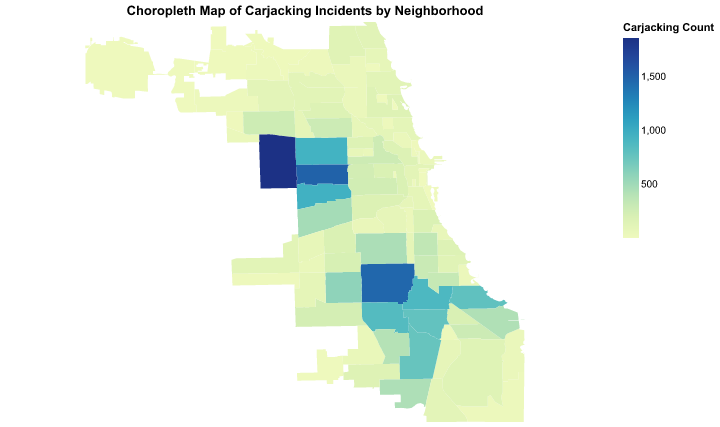
\includegraphics[width=0.5\textwidth,height=\textheight]{pictures/choropleth_map.png}

}

\caption{Choropleth Map of Carjackings}

\end{figure}%

\subsection{2. Line Chart: Carjacking Trends Over
Time}\label{line-chart-carjacking-trends-over-time}

This chart highlights trends in carjacking incidents over time. A sharp
increase is evident around 2020, peaking in 2021. This trend may reflect
broader societal disruptions, such as those caused by the COVID-19
pandemic and economic turmoil. Policymakers could use this data to
explore the impact of external events on crime rates.

\begin{figure}[H]

{\centering 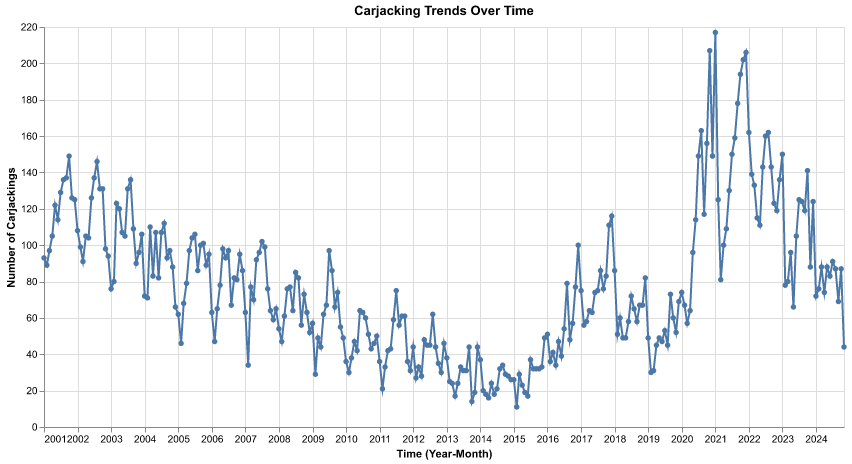
\includegraphics[width=0.5\textwidth,height=\textheight]{pictures/line_chart.png}

}

\caption{Carjacking Trends Over Time}

\end{figure}%

\section{Shiny Dashboard}\label{shiny-dashboard}

The \textbf{Interactive Carjacking Dashboard} enables users to:

\begin{enumerate}
\def\labelenumi{\arabic{enumi}.}
\tightlist
\item
  Explore carjacking patterns dynamically using a \textbf{Choropleth
  Map} filtered by neighborhood and date range.
\item
  Visualize temporal patterns through a \textbf{Line Chart} with
  customizable filters for precise analysis.
\end{enumerate}

\section{Strengths}\label{strengths}

\begin{itemize}
\tightlist
\item
  \textbf{Dynamic Exploration}: Offers flexibility to investigate
  specific neighborhoods or time periods.
\item
  \textbf{Policy Relevance}: Combines spatial and temporal data for
  actionable insights.
\end{itemize}

\section{Weaknesses}\label{weaknesses}

\begin{itemize}
\tightlist
\item
  \textbf{Performance}: Processing large datasets slows responsiveness
\item
  \textbf{Data Limitations}: Missing records in the dataset can affect
  accuracy.
\end{itemize}

\section{Policy Implications}\label{policy-implications}

\subsection{1. Neighborhood Hotspots: Targeted
Interventions}\label{neighborhood-hotspots-targeted-interventions}

Neighborhoods like Austin, West Garfield Park, East Garfield Park,
Englewood, and West Englewood are carjacking hotspots, requiring focused
interventions.

\begin{itemize}
\tightlist
\item
  \textbf{Policy Actions}: Increase police patrols during high-risk
  hours, implement community safety programs like neighborhood watch and
  workshops, improve infrastructure like installing street lighting and
  surveillance cameras, and invest in socioeconomic support like job
  training and education.
\end{itemize}

\subsection{2. Temporal Patterns: Addressing Crime
Spikes}\label{temporal-patterns-addressing-crime-spikes}

The sharp increase in carjackings during 2020-2021 and patterns in
seasons and times of day highlight actionable trends.

\begin{itemize}
\tightlist
\item
  \textbf{Policy Actions}: Allocate law enforcement resources during
  high-crime months and times, and prepare for crime surges during
  external crises such as pandemics or economic crises.
\end{itemize}

\subsection{3. Insurance Policies: Data-Driven
Solutions}\label{insurance-policies-data-driven-solutions}

Car insurance often unfairly penalizes residents of high-crime areas.
Policies should prioritize fairness.

\begin{itemize}
\item
  \textbf{Policy Actions}: Use risk-based pricing focused on individual
  factors, incentivize safety measures such as giving discounts for
  anti-theft devices, require transparency in how crime stats influence
  premiums, and collaborate with law enforcement to lower risks and
  premiums.
\item
  \textbf{Broader Considerations}: Adress poverty and unemployment in
  high-crime neighborhoods, collaborate with residents to foster trust
  and safety, and regularly assess the effectiveness of interventions
  using updated data.
\end{itemize}

\section{Future Directions}\label{future-directions}

Future work should focus on integrating additional datasets, such as
police reports and traffic patterns, to provide deeper insights into
carjacking trends and their underlying causes. Enhancing the dashboard's
interactivity and performance by optimizing data structures will improve
user experience and scalability. Additionally, evaluating the impact of
crime prevention measures through comparative analysis of pre- and
post-intervention data will help assess policy effectiveness and inform
future strategies.

\subsection{Acknowledgement}\label{acknowledgement}

This project was completed for PPHA 30538 under the guidance of
Professors Peter Ganong and Maggie Shi.




\end{document}
